\documentclass[11pt]{article}
\usepackage[a4paper,margin=25mm]{geometry}
\usepackage[T1]{fontenc}
\usepackage{lmodern,microtype}
\usepackage{amsmath,amssymb,amsthm,mathtools}
\usepackage{graphicx}
\usepackage[colorlinks=true,linkcolor=blue,citecolor=blue,urlcolor=blue]{hyperref}

\newtheorem{theorem}{Theorem}
\newtheorem{proposition}[theorem]{Proposition}
\newtheorem{lemma}[theorem]{Lemma}
\newtheorem{corollary}[theorem]{Corollary}
\theoremstyle{remark}
\newtheorem{remark}[theorem]{Remark}

\newcommand{\HH}{\mathcal H}
\newcommand{\E}{\mathbb E}
\newcommand{\dd}{\mathrm d}
\newcommand{\acosh}{\operatorname{arcosh}}
\newcommand{\sgn}{\operatorname{sign}}

\hypersetup{pdftitle={Sharp lower bounds on first-passage skewness and kurtosis in unicyclic networks},pdfauthor={Brandon Li}}

\title{Sharp lower bounds on first-passage skewness\\ and kurtosis in unicyclic networks}
\author{Brandon Li\\[2pt]{\small Great Neck, NY, USA}\\{\small\href{mailto:brandon.li.gn@gmail.com}{\nolinkurl{brandon.li.gn@gmail.com}}}}
\date{}

\begin{document}
\maketitle

\begin{abstract}
Small driven systems such as molecular motors and enzymes run through noisy
reaction cycles, so the time they need to complete a given amount of work
fluctuates. For unicyclic Markov networks with $n$ states and affinity $F$,
Wampler and Barato conjectured sharp lower bounds on the skewness and excess
kurtosis of the first-passage time of entropy production through a large
threshold: the smallest values attained by homogeneous cycles with $m\le n$
states at the same affinity. We prove these conjectures for every $n$ and
every $F>0$, and extend the bound to every standardized cumulant of order
$k\ge3$, where it is expressed through Legendre polynomials. The bounds are
sharp at exactly $n$ states; when a smaller cycle is optimal, they are
approached by making the excess states fast. The optimal number of effective
states is one of two explicit adjacent integers, and it runs through
$1,2,\dots,n$ without skips as $F$ grows. For stationary initial conditions
the large-threshold limit is uniform in the rates. The proof encodes the
passage-time law in a single real polynomial with a band-and-gap structure
and rules out every inhomogeneous minimizer by first- and second-order
variations.
\end{abstract}

\noindent\textit{Keywords}: first-passage times, stochastic thermodynamics,
unicyclic networks, skewness and kurtosis, Chebyshev polynomials

\section{Introduction}

Small driven systems such as molecular motors, chemical clocks and enzymes
operate far from equilibrium through noisy cyclic transitions. In such
systems the fluctuations of time-integrated currents, and of first-passage
times (the waiting times for a current to reach a threshold), are
constrained by the entropy they produce. The thermodynamic uncertainty
relation bounds the relative variance of a current by the inverse entropy
production, and its first-passage version bounds the variance of the time a
current needs to reach a threshold~\cite{gh,garrahan}. For unicyclic
networks the variance bound sharpens to an affinity-dependent
hyperbolic-cotangent bound~\cite{pbs,pbsproof}, attained by homogeneous
cycles, in which all forward rates are equal and all backward rates are
equal.

Beyond the variance, the shape of a first-passage distribution is described
by its skewness and excess kurtosis. For enzymatic cycles with an
irreversible step, Barato and Seifert identified lower bounds on these
quantities~\cite{bs}. Wampler and Barato~\cite{wb} then studied the
first-passage time $T_J$ of entropy production through a threshold $J$ in a
general unicyclic network with $n$ states and affinity $F$. Scaling by the
threshold keeps the statistics finite as $J\to\infty$:
\[
S=\lim_{J\to\infty}J^{1/2}\frac{\kappa_3(T_J)}{\kappa_2(T_J)^{3/2}},\qquad
K=\lim_{J\to\infty}J\,\frac{\kappa_4(T_J)}{\kappa_2(T_J)^{2}},
\]
where $\kappa_j$ denotes the $j$th cumulant. Here $S$ measures the asymmetry
of the passage-time distribution and $K$ the weight of its tails. Based on
extensive numerics, Wampler and Barato conjectured that
\begin{equation}\label{eq:conj}
S\ge\min_{1\le m\le n}f(F/m),\qquad K\ge\min_{1\le m\le n}g(F/m),
\end{equation}
where
\begin{equation}\label{eq:fg}
f(x)=2\sqrt{x}\,\frac{1+4e^x+e^{2x}}{\sqrt{(e^x-1)(1+e^x)^3}},\qquad
g(x)=6x\,\frac{1+8e^x+e^{2x}}{e^{2x}-1}
\end{equation}
are the values of $S$ and $K$ for the homogeneous $m$-state cycle at
affinity $F$, evaluated at the affinity per state
$x=F/m$~\cite[Eqs.~(19)--(22)]{wb}. (The inequality signs printed
in~\cite[Eqs.~(20)--(21)]{wb} are reversed relative to the text and figures,
which describe lower bounds.) In words,~\eqref{eq:conj} says that no
$n$-state ring has a less skewed or lighter-tailed passage-time distribution
than the best homogeneous cycle with at most $n$ states at the same driving
force. Because the best state count $m$ can be strictly less than $n$, the
lower envelope has kinks as $F$ varies. The bounds fail for multicyclic
networks~\cite{wb}. Petkov~\cite{petkov} proved the skewness bound for $n=3$,
together with the large-threshold asymptotics for fixed networks with
$n\ge3$.

In this paper we prove~\eqref{eq:conj} for every $n$ and every $F>0$
(Theorem~\ref{thm:main}). The proof treats all cumulant orders at once: for
every integer $k\ge3$, the affinity-scaled standardized cumulant is bounded
below by the minimum over homogeneous cycles with at most $n$ states
(Theorem~\ref{thm:allorder}). The bounds are sharp at exactly $n$ states. We
also identify the optimal homogeneous branch: at each order $k$ the optimal
state count is one of two adjacent integers near $F/(2z_k)$ for an explicit
constant $z_k$, and it steps through $1,2,\dots,n$ in order as $F$ increases
(Theorem~\ref{thm:selector}). Letting $n\to\infty$ recovers the absolute
lower bounds $S\ge3.9097\ldots$ and $K\ge25.091\ldots$ observed numerically
in~\cite{wb} (Corollary~\ref{cor:absolute}).

Our approach turns the stochastic problem into a variational problem for a
single real polynomial. Combining the inversion relation between currents
and first-passage times~\cite{gh} with the characteristic-polynomial method
of~\cite{wb}, we encode the passage-time law in the spectral polynomial
\[
h(s)=\cosh\frac F2+\frac{\det(sI-Q)}{2\sqrt{PM}},
\]
where $Q$ is the generator and $P,M$ are the products of the forward and
backward rates; $h$ determines the Laplace transform of the time needed to
complete one net forward cycle. Conjugating the tilted generator by a
diagonal matrix makes it Hermitian, so its eigenvalues are real, and this
shows that $h(s)-t$ has only real negative zeros for every $t\in[-1,1]$. All
unicyclic networks therefore lie in a compact class of polynomials whose
inverse image of $[-1,1]$ consists of bands separated by gaps, a structure
studied in the theory of polynomial inverse images and periodic Jacobi
matrices~\cite{totik,ey}. In this class the homogeneous cycles are the
affine Chebyshev polynomials, which oscillate between $-1$ and $1$ with all
gaps closed. We show first that a minimizer has at most one open gap, the
one farthest from the origin, and then exclude that case by a second-order
variation along a curve parametrized by the variance. Sharpness at exactly
$n$ states, when a smaller cycle is optimal, follows by grouping states into
blocks with fast internal transitions.

The paper is organized as follows. Section~\ref{sec:results} defines the
model, states the results and outlines the proof. Section~\ref{sec:poly}
constructs the polynomial class. Section~\ref{sec:gaps} reduces the problem
to one open gap, Section~\ref{sec:homog} treats homogeneous cycles and
sharpness, and Section~\ref{sec:proof} completes the proof of the bounds.
Sections~\ref{sec:selector} and~\ref{sec:threshold} prove the branch
selection theorem and the large-threshold limit.

\section{Model and results}\label{sec:results}

\subsection{Unicyclic networks and period passage}

\begin{figure}[t]
\centering
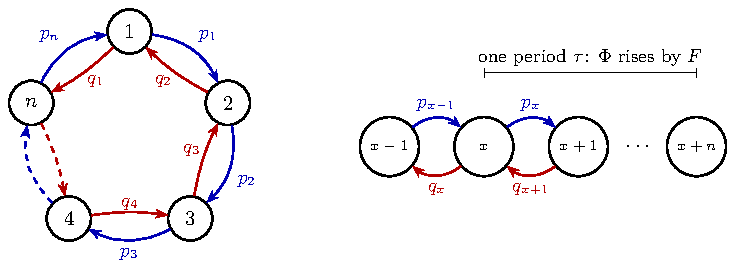
\includegraphics[width=\linewidth]{ring.pdf}
\caption{Left: a unicyclic network with $n$ states, forward rates $p_i$ and
backward rates $q_i$. Right: its lift to $\mathbb Z$, a nearest-neighbor
walk with rates of period $n$. The period passage time $\tau$ is the time
the lifted walk needs to advance $n$ sites, during which the medium-entropy
potential $\Phi$ rises by the affinity $F$.}
\label{fig:ring}
\end{figure}

Consider a continuous-time Markov jump process on a ring of $n\ge1$ states
$i\in\mathbb Z/n\mathbb Z$, which jumps from $i$ to $i+1$ at rate $p_i>0$ and
from $i$ to $i-1$ at rate $q_i>0$ (Figure~\ref{fig:ring}). For $n=2$ the two
channels between the states are kept distinct, and for $n=1$ the process
consists of marked forward and backward events. To track net rotations
around the ring, we lift the process to $\mathbb Z$, obtaining a
nearest-neighbor walk $X_t$ whose rates are periodic with period $n$. The
affinity of the cycle is
\begin{equation}\label{eq:F}
P=\prod_{i=1}^np_i,\qquad M=\prod_{i=1}^nq_i,\qquad F=\log\frac PM,
\end{equation}
and by reversing orientation we assume $F>0$. Physically, $F$ is the
entropy dissipated into the environment per net forward cycle.

A forward jump from $x$ to $x+1$ produces medium entropy
$\log(p_x/q_{x+1})$, and the reverse jump produces its negative. Hence the
accumulated medium entropy is a potential difference $\Phi(X_t)-\Phi(X_0)$
on the lift, with $\Phi(x+n)=\Phi(x)+F$. The entropy first-passage time
through a threshold $J>0$ is
\[
T_J=\inf\{t\ge0:\ \Phi(X_t)-\Phi(X_0)\ge J\}.
\]
Its large-$J$ statistics are governed by the \emph{period passage time}
$\tau$, the first time the lifted walk started at $x$ reaches $x+n$, that
is, the time needed to complete one net forward cycle. The law of $\tau$
does not depend on $x$ (Section~\ref{sec:threshold}), and successive period
passages are independent and identically distributed. The next proposition
shows that each cumulant of $T_J$ grows linearly in the number $J/F$ of
cycles needed, and that for a stationary start the boundary error is bounded
uniformly in the rates.

\begin{proposition}[Large-threshold limit]\label{prop:threshold}
Fix positive rates and any initial phase distribution. For every integer
$j\ge1$,
\[
\kappa_j(T_J)=\frac JF\,\kappa_j(\tau)+O(1)\qquad(J\to\infty).
\]
If the process starts in its stationary distribution, the $O(1)$ term is
bounded uniformly over all positive rates with fixed $n$ and $F$, after
the rates are scaled so that $\E\tau=1$.
\end{proposition}

Dividing by powers of the variance cancels the factors of $J$, so the scaled
skewness and excess kurtosis are single-cycle quantities,
\begin{equation}\label{eq:SK}
S=\sqrt F\,\frac{\kappa_3(\tau)}{\kappa_2(\tau)^{3/2}},\qquad
K=F\,\frac{\kappa_4(\tau)}{\kappa_2(\tau)^2}.
\end{equation}
More generally, for every integer $k\ge3$ we define the affinity-scaled
standardized cumulant
\begin{equation}\label{eq:Ak}
A_k=\lim_{J\to\infty}J^{k/2-1}\frac{\kappa_k(T_J)}{\kappa_2(T_J)^{k/2}}
=F^{k/2-1}\frac{\kappa_k(\tau)}{\kappa_2(\tau)^{k/2}}.
\end{equation}
Thus $A_3=S$ and $A_4=K$. If the threshold counts complete cycles, so that
$T$ is the time to complete $N$ net forward cycles, then $T$ is exactly a sum
of $N$ independent copies of $\tau$, and~\eqref{eq:SK} holds for every $N$
with $J=NF$, not only in the limit. By the uniform part of
Proposition~\ref{prop:threshold}, for stationary initial conditions the
bounds below hold for $J^{k/2-1}\kappa_k(T_J)/\kappa_2(T_J)^{k/2}$ up to a
relative error $O(1/J)$ that is uniform in the rates.

\subsection{Main results}

To state the bounds at every order, let
\begin{equation}\label{eq:Hk}
H_k(j;F)=j^{1-k/2}\,\frac{P_{k-1}(c_j)}{c_j^{k/2}},\qquad
c_j=\coth\frac F{2j},
\end{equation}
for $j>0$ and integer $k\ge3$, where $P_r$ is the Legendre polynomial of
degree $r$. For integer $j$, $(k-1)!\,F^{k/2-1}H_k(j;F)$ is the value of
$A_k$ for the homogeneous $j$-state cycle at affinity $F$
(Section~\ref{sec:homog}).

Our main result says that no $n$-state network has a smaller $A_k$ than the
best homogeneous cycle with at most $n$ states. When that cycle has fewer
than $n$ states, the bound is approached by making the excess states
\emph{fast}: their outgoing rates are sent to infinity, so the walk crosses
them in negligible time.

\begin{theorem}[Lower envelope at every order]\label{thm:allorder}
Let $n\ge1$, $F>0$ and $k\ge3$ an integer. Every unicyclic network with $n$
states and affinity $F$ satisfies
\begin{equation}\label{eq:allorder}
A_k\ \ge\ (k-1)!\,F^{k/2-1}\min_{1\le j\le n}H_k(j;F).
\end{equation}
The bound is the infimum over networks with exactly $n$ states and affinity
exactly $F$. If $j=n$ is a minimizing index, it is attained by the
homogeneous $n$-state cycle. If every minimizing index is smaller than $n$,
the bound is not attained and is approached by $n$-state networks in which
$n-j$ states become fast.
\end{theorem}

For $k=3,4$ the right side of~\eqref{eq:allorder} equals
$\min_jf(F/j)$ and $\min_jg(F/j)$ respectively, which proves the
conjectures of Wampler and Barato.

\begin{theorem}[Skewness and kurtosis]\label{thm:main}
For every $n\ge1$, every $F>0$ and every unicyclic network with $n$ states
and affinity $F$,
\[
S\ \ge\ \min_{1\le m\le n}f(F/m),\qquad K\ \ge\ \min_{1\le m\le n}g(F/m),
\]
with $f,g$ as in~\eqref{eq:fg}. Both bounds are sharp at exactly $n$ states
and affinity $F$, in the sense of Theorem~\ref{thm:allorder}.
\end{theorem}

Which state count achieves the minimum in~\eqref{eq:allorder}? The next
theorem shows that $H_k(j;F)$ has a single valley as a function of $j$,
which pins the optimal branch down to at most two adjacent integers.

\begin{theorem}[Selection of the effective state count]\label{thm:selector}
For each integer $k\ge3$ there is a unique $z_k>0$ such that, for every
$F>0$, the function $j\mapsto H_k(j;F)$ on $(0,\infty)$ strictly decreases on
$(0,F/(2z_k)]$ and strictly increases on $[F/(2z_k),\infty)$. Consequently
the minimizing indices in~\eqref{eq:allorder} lie among
$\lfloor F/(2z_k)\rfloor$ and $\lceil F/(2z_k)\rceil$, clipped to
$\{1,\dots,n\}$.
\end{theorem}

As a consequence, the optimal state count grows one step at a time as the
driving force increases, and each step happens at a single affinity.

\begin{corollary}[Ordered switches]\label{cor:switch}
For fixed $k\ge3$ and each $m\ge1$ there is exactly one affinity
$F_{k,m}\in(2mz_k,2(m+1)z_k)$ at which $H_k(m;F)=H_k(m+1;F)$; for
$F<F_{k,m}$ the $m$-state branch is smaller, and for $F>F_{k,m}$ the
$(m+1)$-state branch is smaller. Hence, for fixed $n$, the optimal effective
state count in~\eqref{eq:allorder} equals $1,2,\dots,n$ in turn as $F$
increases, with ties only between adjacent counts at the affinities
$F_{k,m}$.
\end{corollary}

Numerically, $z_3=1.150671\ldots$ and $z_4=1.320669\ldots$. Since
$(k-1)!F^{k/2-1}H_k(j;F)$ depends on $F$ and $j$ only through the affinity
per state $F/j$, letting $n\to\infty$ removes the restriction on the state
count and gives bounds valid for every unicyclic network.

\begin{corollary}[Absolute bounds]\label{cor:absolute}
For every unicyclic network, $S\ge\min_{x>0}f(x)=3.909729\ldots$, attained
at $x=2z_3$, and $K\ge\min_{x>0}g(x)=25.09134\ldots$, attained at $x=2z_4$.
These constants are the infima over all $n$ and $F$.
\end{corollary}

\begin{remark}[Linear response]\label{rem:linear}
As $F\to0$, every homogeneous branch $(k-1)!\,F^{k/2-1}H_k(j;F)$ tends to
$2^{k/2-1}(2k-3)!!$, because $c_j\sim2j/F$ and
$P_{k-1}(c)\sim\binom{2k-2}{k-1}(c/2)^{k-1}$; hence so does the envelope for
every $n$. This gives $S\to3\sqrt2$ and $K\to30$, the values for the first
passage of a drifted Brownian motion (an inverse Gaussian law) with
mean-to-shape ratio $2/F$. Close to equilibrium the bound therefore does not
depend on the network size; the dependence on $n$ appears only at finite
affinity.
\end{remark}

Figure~\ref{fig:envelope} shows the envelopes. The kinks found numerically
in~\cite{wb} are the switching affinities $F_{k,m}$ of
Corollary~\ref{cor:switch}. Figure~\ref{fig:random} compares the bound with
randomly sampled three-state rings.

\begin{figure}[t]
\centering
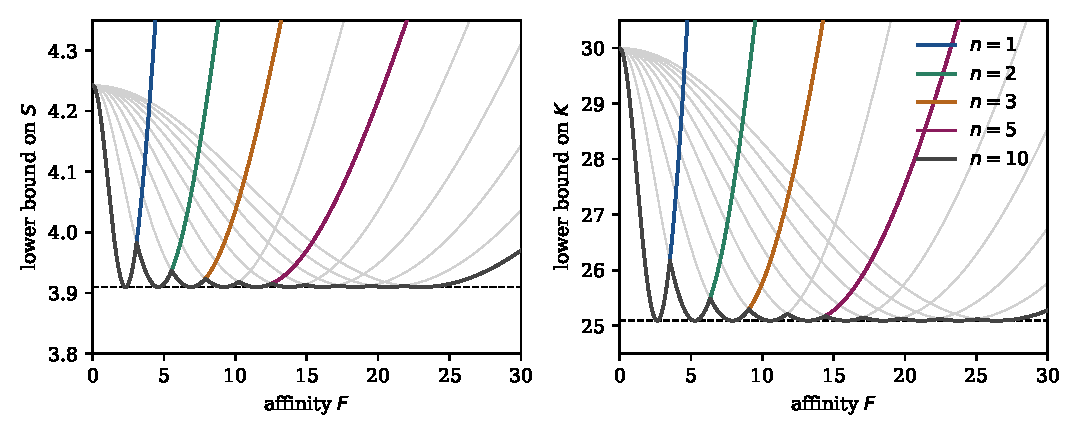
\includegraphics[width=\linewidth]{envelope.pdf}
\caption{Sharp lower envelopes of the scaled skewness $S$ (left) and excess
kurtosis $K$ (right) as functions of the affinity $F$, for $n=1,2,3,5,10$
states (solid). Each envelope is the minimum of the homogeneous branches
$f(F/m)$, $g(F/m)$ with $m\le n$ (thin gray, $m=1,\dots,10$). The dashed
lines are the absolute minima of Corollary~\ref{cor:absolute}.}
\label{fig:envelope}
\end{figure}

\begin{figure}[t]
\centering
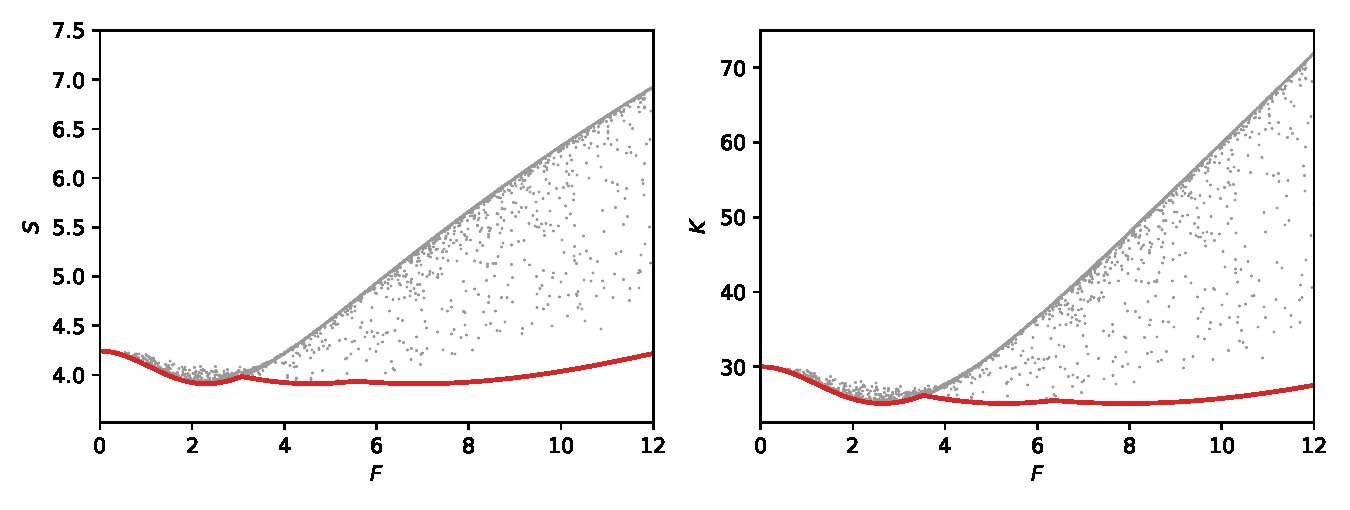
\includegraphics[width=\linewidth]{random.pdf}
\caption{Scaled skewness $S$ (left) and excess kurtosis $K$ (right) of 4000
three-state rings with rates drawn log-uniformly from $[10^{-3},10^3]$
(gray), against the lower envelope of Theorem~\ref{thm:main} for $n=3$
(red). Every sampled ring lies on or above the envelope.}
\label{fig:random}
\end{figure}

\subsection{Strategy of the proof}\label{sec:strategy}

\begin{figure}[!htb]
\centering
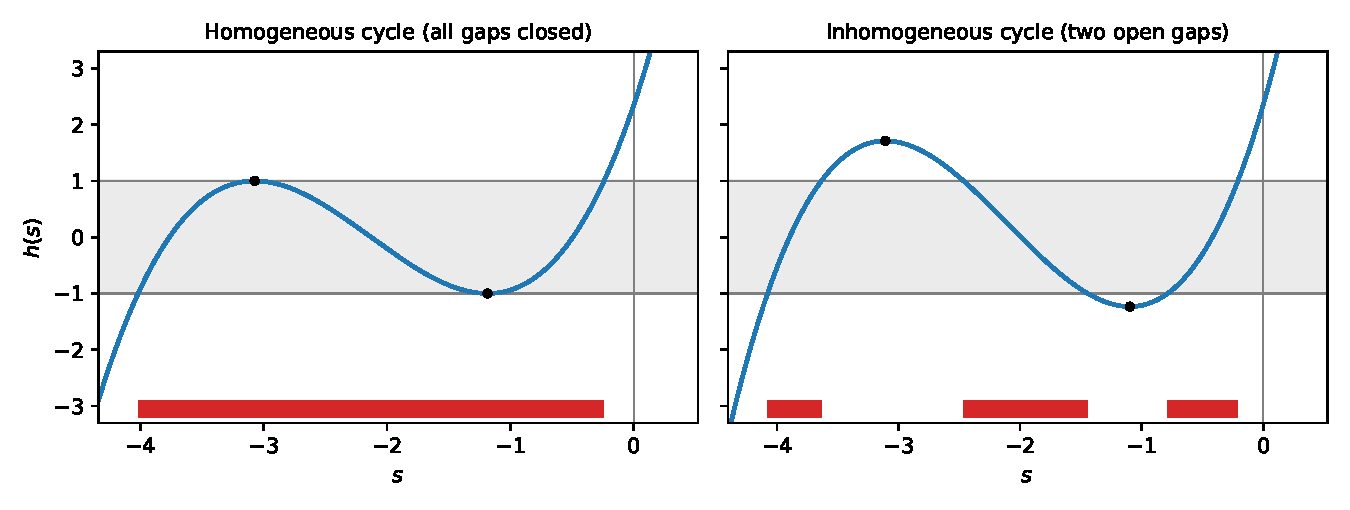
\includegraphics[width=\linewidth]{bands.pdf}
\caption{Spectral polynomials $h(s)$ of two three-state rings at $F=3$. The
gray strip is $|h|\le1$; the red intervals on the $s$ axis are the bands,
and the dots mark the critical points. Left: the homogeneous cycle, whose
critical values are exactly $\pm1$, so all gaps are closed and the bands
touch. Right: an inhomogeneous cycle, whose critical values exceed $1$ in
modulus, so both gaps are open.}
\label{fig:bands}
\end{figure}

Every $n$-state network is encoded in the degree-$n$ spectral polynomial
$h(s)$ of~\eqref{eq:h}. The set of real $s$ with $-1\le h(s)\le1$ splits into
closed intervals called \emph{bands}, separated by open intervals called
\emph{gaps} (Figure~\ref{fig:bands}). Between two consecutive bands $h$ has a
critical point where $|h|\ge1$; the gap is \emph{closed} when $|h|=1$ there,
so the neighboring bands touch, and \emph{open} otherwise. The Hermitian
structure mentioned above puts every band on the negative real axis.

Within this class, the homogeneous cycles are exactly the polynomials with
every gap closed: these are the affine Chebyshev polynomials, whose local
extrema all lie at $\pm1$. The task is therefore to show that a minimizer of
$A_k$ has no open gap.

To minimize $A_k$ we vary the critical values of $h$. First-order
optimality conditions show that a minimizer has at most one open gap, and
that this gap, if present, is the leftmost one, farthest from the origin.

We rule out this last case with a second-order argument. From such a
candidate we deform $h$ along a smooth curve that keeps every closed gap
closed and uses the variance as its parameter. Along this curve, every
critical point of $A_k$ with one open gap is a strict local maximum, never
a minimum. Hence every minimizer has all gaps closed and is a homogeneous
cycle of some size $m\le n$.

Finally, when the optimal homogeneous cycle has fewer than $n$ states, we
approach its bound with exactly $n$ states and affinity $F$ by grouping the
ring into $m$ blocks of consecutive states. Sending the rates inside each
block to infinity makes each block equilibrate almost instantly, so it
behaves as a single effective state.

\section{The spectral polynomial}\label{sec:poly}

\subsection{The period transform}
We begin by encoding the dynamics of the ring in a single polynomial. Let
$Q$ be the generator of the projected $n$-state chain (summing the two
channels when $n=2$, and setting $Q=0$ when $n=1$). We define
\begin{equation}\label{eq:h}
C=\cosh\frac F2,\qquad D=\sinh\frac F2,\qquad
h(s)=C+\frac{\det(sI-Q)}{2\sqrt{PM}}.
\end{equation}
Here $h(s)$ is a real polynomial of degree $n$ that combines the spectrum of
the generator with the driving force $F$. Tilting the forward rates by $z$
and the backward rates by $z^{-1}$ gives the standard
identity~\cite{wb}
\begin{equation}\label{eq:tilt}
\det(sI-Q(z))=\det(sI-Q)+P+M-Pz-Mz^{-1},
\end{equation}
which is interpreted as $s+p_1+q_1-p_1z-q_1z^{-1}$ for $n=1$.

The next lemma links this polynomial to the period passage time $\tau$: it
gives the cumulant generating function of $\tau$ in closed form in terms of
$h$. This turns the probabilistic problem of bounding cumulants of $\tau$
into an analytic problem about $h$.

\begin{lemma}\label{lem:transform}
The Laplace exponent $\gamma(s)=-\log\E e^{-s\tau}$ is analytic near $s=0$
and satisfies
\begin{equation}\label{eq:gamma}
\gamma(s)=\acosh h(s)-\frac F2,\qquad
\kappa_j(\tau)=(-1)^{j-1}\gamma^{(j)}(0).
\end{equation}
\end{lemma}

\begin{proof}
We construct a martingale of the form $e^{-st}\phi_s(X_t)$ on the lifted
walk and stop it at $\tau$. For a function $\phi$ on $\mathbb Z$, the
equation $p_x\phi(x+1)-(s+p_x+q_x)\phi(x)+q_x\phi(x-1)=0$ is a periodic
second-order recurrence. Propagating $(\phi(x),\phi(x-1))$ across one
period defines a $2\times2$ transfer matrix, whose determinant is $M/P$ and
whose trace is $[\det(sI-Q)+P+M]/P$ by~\eqref{eq:tilt}. Its eigenvalues,
the Floquet multipliers $z$ (the factor by which a quasi-periodic solution
is multiplied over one period), therefore solve
$Pz+Mz^{-1}=\det(sI-Q)+P+M$.

At $s=0$ the two multipliers are $1$ and $M/P<1$, so the multiplier $z(s)$
with $z(0)=1$ is simple and analytic near $s=0$. For small $s>0$ the
corresponding Floquet solution $\phi_s$ is positive, satisfies
$\phi_s(x+n)=z(s)\phi_s(x)$ with $z(s)>1$, and is bounded on the half-line
to the left of the target. Optional stopping of the bounded martingale
$e^{-st}\phi_s(X_t)$ at $\tau$ gives $\E e^{-s\tau}=z(s)^{-1}$.

For small $s<0$ the continued solution is positive with $z(s)<1$ and
bounded below on that half-line, so the stopped supermartingale bounds
$\E e^{|s|(\tau\wedge t)}$ uniformly in $t$. Hence $\tau$ has exponential
moments, and the identity extends analytically across $s=0$. Writing
$z=e^{\gamma}$, the multiplier equation becomes
$\sqrt{PM}\,(e^{\gamma+F/2}+e^{-\gamma-F/2})=\det(sI-Q)+P+M$, that is,
$\cosh(\gamma+F/2)=h(s)$, with $\gamma(0)=0$.
\end{proof}

Multiplying all rates by a positive constant rescales time without changing
$A_k$ or $F$. We therefore normalize the mean cycle time to
$\E\tau=\gamma'(0)=1$, which is equivalent to
\begin{equation}\label{eq:normal}
h(0)=C,\qquad h'(0)=D.
\end{equation}

Not every polynomial can arise from a Markov ring. The next lemma gives the
spectral constraint shared by all networks: every level set $h(s)=t$ with
$t\in[-1,1]$ lies on the negative real axis. This constraint is what gives
$h$ its band-and-gap structure.

\begin{lemma}\label{lem:physical}
For every positive-rate network and every $t\in[-1,1]$, all zeros of
$h(s)-t$ are real and strictly negative.
\end{lemma}

\begin{proof}
We realize the zeros of $h(s)-t$ as the negatives of the eigenvalues of a
positive definite Hermitian matrix. Let $t=\cos\theta$ and
$z=e^{-F/2+i\theta}$. Distributing the tilt over the edges and conjugating
by a diagonal matrix turns $-Q(z)$ into a Hermitian cyclic Jacobi matrix
$H_\theta$, a tridiagonal matrix with corner entries closing the ring, like
a tight-binding Hamiltonian on a ring. Indeed, the forward and backward
products of its off-diagonal entries are $Pz=\sqrt{PM}e^{i\theta}$ and
$Mz^{-1}=\sqrt{PM}e^{-i\theta}$, which are complex conjugates. Its
quadratic form is a sum of squares,
\[
\langle v,H_\theta v\rangle=\sum_{i=1}^n
\bigl|\sqrt{p_i}\,v_i-e^{i\phi_i}\sqrt{q_{i+1}}\,v_{i+1}\bigr|^2,
\qquad\sum_i\phi_i=\theta,
\]
with cyclic indices; for $n=2$ both edges are kept and for $n=1$ the sum is a
single term. A nonzero kernel vector would satisfy
$\sqrt{p_i}\,v_i=e^{i\phi_i}\sqrt{q_{i+1}}\,v_{i+1}$ for all $i$, hence all
$v_i\neq0$, and multiplying these relations around the ring gives
$e^{F/2}=e^{i\theta}$, which is impossible because $F>0$. So $H_\theta$ is
positive definite. By~\eqref{eq:tilt},
$\det(sI+H_\theta)=\det(sI-Q)+P+M-2\sqrt{PM}\cos\theta=2\sqrt{PM}\,[h(s)-t]$,
so the zeros of $h-t$ are the negatives of the eigenvalues of $H_\theta$.
\end{proof}

\subsection{The polynomial class}
We now replace the optimization over rates by an optimization over
polynomials. Let $\HH_n$ be the set of real polynomials $h$ of degree
between $1$ and $n$ that satisfy~\eqref{eq:normal} and the conclusion of
Lemma~\ref{lem:physical}. By Lemmas~\ref{lem:transform}
and~\ref{lem:physical}, the normalized polynomial of every $n$-state network
lies in $\HH_n$ and has degree exactly $n$. We never need the converse: the
lower bound is proved on the larger set $\HH_n$, and sharpness is proved by
explicit networks in Section~\ref{sec:homog}.

To know that a minimizing polynomial exists and to describe small
deformations of it, we need the geometry of $\HH_n$. The next lemma shows
that $\HH_n$ is compact and that, locally, membership in $\HH_n$ is a set
of simple inequalities on the critical values of $h$.

\begin{lemma}\label{lem:compact}
$\HH_n$ is compact in coefficient space. A member of degree $m$ has $m$
simple negative zeros and $m-1$ distinct negative critical points
$x_1<\dots<x_{m-1}$, at which
\begin{equation}\label{eq:gaps}
\sigma_ih(x_i)\ge1,\qquad\sigma_i=(-1)^{m-i}.
\end{equation}
Conversely, near a member of degree $m$, a polynomial of degree $m$
satisfying~\eqref{eq:normal} lies in $\HH_n$ if and only if it
satisfies~\eqref{eq:gaps}.
\end{lemma}

Geometrically, \eqref{eq:gaps} says that between consecutive bands the
polynomial reaches or passes $\pm1$. We call the gap at $x_i$
\emph{closed} if equality holds in~\eqref{eq:gaps}, and \emph{open}
otherwise. A closed gap is a double zero of $h-1$ or $h+1$.

\begin{proof}
For compactness we parametrize $h$ by its zeros. At level zero write
$h(s)=C\prod_{i=1}^m(1+u_is)$ with $u_i>0$; then $\sum_iu_i=D/C$
by~\eqref{eq:normal}. Padding with zeros embeds all degrees in the compact
simplex $\{u\in[0,\infty)^n:\sum u_i=D/C\}$, and the coefficients are
continuous in $u$. For each $t\in[-1,1]$, real-rootedness of $h-t$ is
preserved under coefficient limits (zeros may escape to infinity), and no
limiting zero can be nonnegative, since $h-t$ has nonnegative coefficients
and constant term $C-t>0$. The degree cannot drop to zero because
$h'(0)=D>0$. Hence $\HH_n$ is closed in a compact set.

Next we describe the critical points. If $h-t$ had a multiple zero for some
$-1<t<1$, a small change of level in one direction would create nonreal
zeros. So the zeros at level $0$ are simple, and by Rolle's theorem (a zero
of $h'$ lies between any two zeros of $h$) the $m-1$ zeros of $h'$ are
simple, real and interlaced with them. The level sets of $h$ in $[-1,1]$
consist of $m$ real points exactly when the critical values alternate in
sign with modulus at least $1$, with the rightmost critical point a
minimum; this is~\eqref{eq:gaps}. The same description holds for nearby
polynomials of the same degree, since critical points depend smoothly on
the coefficients.
\end{proof}

The next lemma writes the cumulants of $\tau$ as inverse moments of a
positive measure. This representation bounds the variance away from zero
and makes the objective continuous on $\HH_n$.

\begin{lemma}\label{lem:moments}
For $h\in\HH_n$ of degree $m$ there is a positive measure $\mu$ on
$[\lambda_*,\infty)$, $\lambda_*=(C-1)/D>0$, with total mass $m$, such that
\begin{equation}\label{eq:Mj}
M_j:=\frac{(-1)^{j-1}\gamma^{(j)}(0)}{(j-1)!}=\int\lambda^{-j}\,\dd\mu(\lambda)
\qquad(j\ge1).
\end{equation}
In particular $M_1=1$, $v:=M_2\ge1/m\ge1/n$, and each $M_j$ is a
continuous function on $\HH_n$.
\end{lemma}

\begin{proof}
We average over the Bloch angle $\theta$ to express $\gamma$ through the
zeros of $h-\cos\theta$. For $s$ near $0$,
\[
\gamma(s)=\frac1{2\pi}\int_0^{2\pi}\log\frac{h(s)-\cos\theta}{C-\cos\theta}\,
\dd\theta=\frac1{2\pi}\int_0^{2\pi}\sum_{i=1}^m
\log\Bigl(1+\frac s{\lambda_i(\theta)}\Bigr)\dd\theta,
\]
where $-\lambda_i(\theta)<0$ are the zeros of $h-\cos\theta$. The first
equality is the identity
$\frac1{2\pi}\int_0^{2\pi}\log(a-\cos\theta)\,\dd\theta=\acosh a-\log2$ for
$a>1$. Differentiating $h-\cos\theta=(C-\cos\theta)\prod_i(1+s/\lambda_i)$
at $s=0$ gives $\sum_i\lambda_i(\theta)^{-1}=D/(C-\cos\theta)\le D/(C-1)$,
so every $\lambda_i(\theta)\ge\lambda_*$. Expanding the logarithm gives
\eqref{eq:Mj} with $\mu$ the pushforward of $\frac{\dd\theta}{2\pi}$ under
the $m$ root branches. Cauchy--Schwarz gives $1=M_1^2\le M_0M_2=mv$.
Continuity follows from~\eqref{eq:gamma}, since $h(0)=C>1$ keeps $\acosh$
analytic near $s=0$ uniformly on the compact class.
\end{proof}

In terms of~\eqref{eq:Mj}, $\kappa_j(\tau)=(j-1)!\,M_j$ and
\begin{equation}\label{eq:Qk}
A_k=(k-1)!\,F^{k/2-1}\,Q_k,\qquad Q_k=\frac{M_k}{v^{k/2}}.
\end{equation}
Minimizing $A_k$ is therefore the same as minimizing the dimensionless
ratio $Q_k$. By Lemmas~\ref{lem:compact} and~\ref{lem:moments}, $Q_k$ is
continuous on the compact set $\HH_n$ and attains its minimum. The core of
the proof is the following classification: only the gapless (homogeneous)
polynomials minimize $Q_k$.

\begin{theorem}\label{thm:poly}
Let $k\ge3$ and $n\ge1$. Every minimizer of $Q_k$ on $\HH_n$ is one of the
homogeneous polynomials $h_1,\dots,h_n$ of~\eqref{eq:cheb}.
\end{theorem}

\section{Reduction to one open gap}\label{sec:gaps}

In this section we use first-order variations to show that a minimizer of
$Q_k$ that is not homogeneous has exactly one open gap, the one farthest
from the origin.

Throughout this section $h\in\HH_n$ has degree $m$, and variations are taken
in the affine space $\{C+Ds+\sum_{j=2}^ma_js^j\}$ of polynomials of degree at
most $m$ satisfying~\eqref{eq:normal}. A minimizer over $\HH_n$ is in
particular a local minimizer in this space, including when $m<n$. Every
variation has the form $\delta h=s^2p$ with $p$ of degree at most $m-2$.
At a critical point $x_i$ the first variation of the critical value is
$\delta h(x_i)$, since $h'(x_i)=0$.

The next lemma turns local optimality into a linear identity for the first
variation of $Q_k$, with nonnegative multipliers on the closed gaps. We
then test it on well-chosen directions.

\begin{lemma}[First-order conditions]\label{lem:kkt}
Let $h$ be a local minimizer of $Q_k$ and let $I$ be the set of indices of
closed gaps. Write $L(p)$ for the first variation of $Q_k$ in the direction
$\delta h=s^2p$. Then there are $\lambda_i\ge0$, $i\in I$, with
\begin{equation}\label{eq:kkt}
L(p)=\sum_{i\in I}\lambda_i\,\sigma_i\,x_i^2\,p(x_i)\qquad
\text{for all }p\in\mathbb R_{m-2}[s].
\end{equation}
\end{lemma}

\begin{proof}
By Lemma~\ref{lem:compact}, near $h$ the class is cut out by the smooth
inequalities $\sigma_ih(x_i(h))\ge1$, $i\in I$, the open gaps being
inactive constraints. Their differentials are $p\mapsto x_i^2p(x_i)$. Since
$|I|\le m-1=\dim\mathbb R_{m-2}[s]$ and the $x_i$ are distinct and nonzero,
Lagrange interpolation (a polynomial of degree at most $m-2$ can take any
prescribed values at $m-1$ distinct points) shows that these functionals
are linearly independent. This is the linear independence constraint
qualification, the regularity condition under which the
Karush--Kuhn--Tucker conditions, the standard first-order conditions for
minimization under inequality constraints, are necessary. These conditions
are~\eqref{eq:kkt}.
\end{proof}

To evaluate $L(p)$ we express the variation of $\gamma$ through $\delta h$.
Varying $\cosh(\gamma+F/2)=h$ gives
\[
\delta\gamma=\frac{\delta h}{\sqrt{h^2-1}}=\frac{\delta h}{h'}\,\gamma',
\qquad \gamma'(s)=\sum_{j\ge0}(-1)^jM_{j+1}s^j,
\]
and the series for $\gamma'$ has strictly alternating coefficients, since
every $M_{j+1}>0$. We repeatedly use the following elementary fact: if
$a(s)=\sum(-1)^ja_js^j$ and $b(s)=\sum(-1)^jb_js^j$ with all $a_j,b_j>0$,
then $ab$ has the same form. For $\rho>0$, $1/(1+s/\rho)$ has this form.

\begin{lemma}[Gap reduction]\label{lem:gap}
Let $k\ge3$. A local minimizer of $Q_k$ that is not a Chebyshev polynomial
(all gaps closed) has exactly one open gap, located at its leftmost
critical point $x_1$.
\end{lemma}

\begin{proof}
In both cases below we choose a direction $\delta h$ that leaves the
variance unchanged and compare the sign of $\delta M_k$
with~\eqref{eq:kkt}.

\emph{Two open gaps.} Suppose $r<t<0$ are open critical points, and let
\[
\delta h=\frac{s^3\,h'(s)}{(s-r)(s-t)}.
\]
Since $r$ and $t$ are zeros of $h'$, this is a polynomial of the form
$s^2p$ with $\deg p\le m-2$, and it vanishes at every closed critical
point, so the right side of~\eqref{eq:kkt} is zero. On the other hand
$\delta\gamma=s^3\gamma'/((s-r)(s-t))$ starts at order $s^3$, so the
variance $v=M_2$ is unchanged, and
\[
\delta M_k=(-1)^{k-1}k\,[s^k]\delta\gamma
=(-1)^{k-1}k\,[s^{k-3}]\frac{\gamma'(s)}{rt\,(1-s/r)(1-s/t)}.
\]
Since $r,t<0$, the fraction has strictly alternating coefficients and
$rt>0$, so $[s^{k-3}]$ has sign $(-1)^{k-3}$ and $\delta M_k>0$. Thus
$L(p)=\delta M_k/v^{k/2}\ne0$, contradicting~\eqref{eq:kkt}.

\emph{One open gap.} Let $r$ be the only open critical point and
$y_1<\dots<y_{m-2}$ the closed ones. Put $G(s)=\prod_i(s-y_i)$, so that
$h'(s)=D(1-s/r)G(s)/G(0)$. Testing~\eqref{eq:kkt} with $p=G$ gives
$L(G)=0$. Let $\ell_i$ be the Lagrange basis polynomial of degree $m-3$ with
$\ell_i(y_j)=\delta_{ij}$. Then~\eqref{eq:kkt} gives
$L(\ell_i)=\lambda_i\sigma(y_i)y_i^2$, where $\sigma(y_i)$ is the sign
in~\eqref{eq:gaps} attached to $y_i$. Since $L(G)=0$, we may add a multiple
of $G$ to $\ell_i$ so that the variation starts at order $s^3$:
\[
L(\ell_i)=L(p_i),\qquad
p_i=\ell_i+\frac{G}{y_iG'(y_i)}=\frac{s\,G(s)}{y_iG'(y_i)(s-y_i)}.
\]
The direction $\delta h=s^2p_i$ gives
\[
\delta\gamma=\frac{s^3G(s)\gamma'(s)}{y_iG'(y_i)(s-y_i)h'(s)}
=\frac{G(0)}{D\,y_iG'(y_i)}\cdot
\frac{s^3\gamma'(s)}{(1-s/r)(s-y_i)}.
\]
Again $v$ is unchanged. With $s-y_i=|y_i|(1+s/|y_i|)$ and $r<0$, the last
fraction is $s^3/|y_i|$ times a series with strictly alternating
coefficients, so as before
\[
\sgn\delta M_k=\sgn\frac{G(0)}{y_iG'(y_i)}=-\sgn G'(y_i)=(-1)^{m-1-i},
\]
using $G(0)=\prod_j|y_j|>0$, $y_i<0$, and the fact that $G'(y_i)$ has the
sign $(-1)^{m-2-i}$ of the number of zeros of $G$ to the right of $y_i$. In
particular $L(\ell_i)\ne0$, so $\lambda_i>0$ and $\sigma(y_i)=(-1)^{m-1-i}$.
If $y_i<r$, then $y_i$ is the $i$th critical point overall and
$\sigma(y_i)=(-1)^{m-i}$, a contradiction. Hence every closed critical point
lies to the right of $r$, and $r=x_1$.
\end{proof}

\subsection{The one-gap flow}
To exclude the remaining case, one open gap at the leftmost critical point,
we deform $h$ along a curve that keeps every closed gap closed. Let $h$ have
exactly one open gap, at $r=x_1=-R$, and closed critical points
$y_1<\dots<y_{m-2}$ in $(-R,0)$. Consider the flow
\begin{equation}\label{eq:flow}
\dot h=-\frac{s^2h'(s)}{s-r}=\frac{D}{r\,G(0)}\,s^2G(s).
\end{equation}
It preserves~\eqref{eq:normal}, the degree, and the value of $h$ at each
closed critical point (since $\dot h(y_i)=0$ and $h'(y_i)=0$, the critical
values $h(y_i(t))$ are constant). For small times the open gap stays open,
so~\eqref{eq:flow} defines a curve in $\HH_n$ through $h$ in both
directions.

Differentiating $h'(r)=0$ along the flow gives
$\dot r=r\,(2+rG'(r)/G(r))$, that is,
\begin{equation}\label{eq:Rdot}
\dot R=R\,(2+\eta),\qquad
\eta=\sum_{i=1}^{m-2}\frac R{R+y_i}.
\end{equation}
Each term exceeds $1$ because $-R<y_i<0$, so $\eta>m-2$ for $m\ge3$, and
$\eta=0$ for $m=2$. Expanding $\dot\gamma=-s^2\gamma'(s)/(s+R)$ in powers
of $s$ gives
\begin{equation}\label{eq:Mdot}
\dot M_j=j\sum_{i=1}^{j-1}\frac{M_i}{R^{\,j-i}},\qquad\text{in particular}\qquad
\dot v=\frac2R>0.
\end{equation}
Since $\dot v>0$, the variance increases along the flow and serves as a
two-sided coordinate on the curve. We write $'$ for $\dd/\dd v$ and $q=1/R$.
Dividing~\eqref{eq:Rdot} and~\eqref{eq:Mdot} by $\dot v=2q$ gives
\begin{equation}\label{eq:vflow}
q'=-1-\frac\eta2,\qquad
M_j'=\frac j2\sum_{i=1}^{j-1}M_iq^{\,j-1-i}.
\end{equation}

On this curve the closed critical points cancel between $h'$ and
$\sqrt{h^2-1}$ in $\gamma'=h'/\sqrt{h^2-1}$, since each is a double zero of
$h^2-1$. The four remaining simple zeros of $h^2-1$ are the two outer band
edges and the two ends of the open gap. Writing them as $-1/x_i$ and using
$\gamma'(0)=1$,
\begin{equation}\label{eq:quartic}
\gamma'(-t)=\frac{1-qt}{\sqrt{\mathcal P(t)}},\qquad
\mathcal P(t)=\prod_{i=1}^4(1-x_it),\qquad
0<x_1<x_2<q<x_3<x_4.
\end{equation}
Here $x_1,x_2$ come from the left outer edge and the left end of the gap,
and $x_3,x_4$ from the right end of the gap and the right outer edge.

To follow $Q_k$ along the flow, let $G(t)=\mathcal P(t)^{-1/2}=\sum_{r\ge0}f_rt^r$
and $c=\frac12\sum_ix_i$. Comparing $\gamma'(-t)=\sum_jM_jt^{j-1}$
with~\eqref{eq:quartic} gives $M_j=f_{j-1}-qf_{j-2}$, and in particular
$c=v+q$ from the coefficient of $t$. Summing~\eqref{eq:vflow} as a geometric
series gives, for $H(t)=(1-qt)G(t)=\sum_jM_jt^{j-1}$,
\begin{equation}\label{eq:Hv}
H'=tG+\tfrac12t^2\partial_tG,\qquad\text{equivalently}\qquad
(1-qt)\,\mathcal P'=\eta\,t\,\mathcal P+\tfrac12t^2\partial_t\mathcal P,
\end{equation}
where $\mathcal P'$ is the derivative with respect to $v$ at fixed $t$, and
$c'=1+q'=-\eta/2$. Finally, $M_k'=\frac k2f_{k-2}$ and
\begin{equation}\label{eq:Ek}
Q_k'=-\frac{k\,E_k}{2v^{k/2+1}},\qquad
E_k=M_k-\frac{2v}kM_k'=f_{k-1}-cf_{k-2}=[t^{k-1}]\,(1-ct)G(t).
\end{equation}
Thus $Q_k$ is stationary along the flow exactly when $E_k=0$. The next lemma
shows that this can only happen when $x_4>c$; Section~\ref{sec:proof} uses
this to find the sign of $Q_k''$.

\begin{lemma}[Localization]\label{lem:local}
If $x_4\le c$, then $E_k<0$ for every $k\ge2$.
\end{lemma}

\begin{proof}
Using $\partial_tG/G=\frac12\sum_ix_i/(1-x_it)$ and $\sum_ix_i=2c$,
\[
\partial_t\bigl[(1-ct)G(t)\bigr]=\frac{t\,G(t)}2\sum_{i=1}^4
\frac{x_i(x_i-c)}{1-x_it}.
\]
If $x_4\le c$ then every $x_i-c\le0$, with strict inequality for $i\le3$.
Since $G$ and each $1/(1-x_it)$ have positive coefficients, every
coefficient of $t^r$, $r\ge1$, on the right is negative. Hence
$[t^{k-1}](1-ct)G<0$ for $k\ge2$.
\end{proof}

\section{Homogeneous cycles and sharpness}\label{sec:homog}

In this section we identify the gapless members of $\HH_n$ as homogeneous
cycles, and we show that every smaller homogeneous cycle can be approached
by networks with exactly $n$ states.

If all gaps of a degree-$m$ member of $\HH_n$ are closed, the $m-1$ critical
points are double zeros of $h^2-1$, and the two remaining zeros are the outer
band edges $a<b<0$. Comparing leading coefficients,
$h^2-1=m^{-2}(s-a)(s-b)h'^2$, and integrating to the right of $b$ shows that
$h$ is an affine Chebyshev polynomial, that is, a Chebyshev polynomial
composed with an affine change of the variable $s$, so that all its local
extrema on $[a,b]$ equal $\pm1$. The normalization~\eqref{eq:normal}
then fixes
\begin{equation}\label{eq:cheb}
h_m(s)=T_m\Bigl(\cosh\theta+\frac sm\sinh\theta\Bigr),\qquad
\theta=\frac F{2m},
\end{equation}
where $T_m(\cosh z)=\cosh(mz)$. This is the spectral polynomial of the
homogeneous $m$-state cycle at affinity $F$, and
$\gamma_m(s)=m\acosh(\cosh\theta+\frac sm\sinh\theta)-F/2$. Therefore
\[
\gamma_m'(-t)=\Bigl(1-\frac{2c_mt}m+\frac{t^2}{m^2}\Bigr)^{-1/2},\qquad
c_m=\coth\theta,
\]
and the generating function of the Legendre polynomials gives
\begin{equation}\label{eq:homM}
M_k(h_m)=m^{-(k-1)}P_{k-1}(c_m),\qquad
Q_k(h_m)=H_k(m;F).
\end{equation}
For $k=3,4$ this gives $A_3=f(F/m)$ and $A_4=g(F/m)$,
reproducing~\eqref{eq:fg}.

The next lemma shows that the bound of a homogeneous cycle with $m<n$
states is still sharp for networks with exactly $n$ states and affinity
$F$. This is what makes the minimum over $1\le m\le n$ in
Theorem~\ref{thm:allorder} an infimum rather than only a lower bound.

\begin{lemma}[Sharpness at exactly $n$ states]\label{lem:sharp}
Let $1\le m\le n$. There are networks with exactly $n$ states and affinity
$F$ whose normalized spectral polynomials converge to $h_m$ in coefficient
space. Along them every $A_k$ converges to its value at $h_m$.
\end{lemma}

\begin{proof}
We group the $n$ states into $m$ consecutive blocks and make the
transitions inside each block fast, so that each block equilibrates almost
instantly and acts as a single effective state. Partition the ring into $m$
consecutive blocks of lengths $L_1,\dots,L_m\ge1$ with $\sum L_i=n$. On
each edge inside a block put rate $R$ in both directions. From the last
state of block $i$ to the first state of block $i+1$ put forward rate
$L_ia$, and from the first state of block $i$ to the last state of block
$i-1$ put backward rate $L_ib$, where $a/b=e^{F/m}$. Then
$P_R/M_R=(a/b)^m=e^F$ for every $R>0$, so the affinity is fixed.

Write $Q_R=RA+B$, where $A$ is the block-diagonal negative Laplacian of the
internal edges. In an orthonormal basis consisting of the normalized block
indicators followed by a basis of their orthogonal complement, the matrix
$sI-Q_R$ splits into a slow (between-block) and a fast (within-block) part,
\[
sI-Q_R=\begin{pmatrix}sI_m-B_{00}&-B_{01}\\-B_{10}&R\Lambda+sI-B_{11}
\end{pmatrix},
\]
with $\Lambda$ positive definite and $\det\Lambda=\prod_iL_i$. On every
fixed disk $|s|\le\rho$, $(R\Lambda+sI-B_{11})^{-1}=R^{-1}\Lambda^{-1}
+O(R^{-2})$. The Schur complement formula, which writes the determinant of
a block matrix as the determinant of the fast block times that of an
effective matrix on the slow block, then gives
$\det(sI-Q_R)=R^{n-m}\prod_iL_i\,[\det(sI-B_{00})+O(R^{-1})]$ uniformly.

Averaging the boundary rates over each block gives
$B_{00}=\Sigma Q_m\Sigma^{-1}$ with $\Sigma=\operatorname{diag}(\sqrt{L_i})$,
where $Q_m$ is the generator of the homogeneous $m$-state cycle with rates
$a,b$. Because $\sqrt{P_RM_R}=R^{n-m}\prod_iL_i\,(ab)^{m/2}$, the
polynomials~\eqref{eq:h} converge uniformly on the disk to that of the
homogeneous cycle. On a small disk about $0$ the limit stays near $C>1$, so
the same branch of $\acosh$ applies. By the Cauchy estimates, uniform
convergence of analytic functions on a disk implies convergence of all
their derivatives at its center, so every derivative of $\gamma$ at $0$
converges. After rescaling time to $\E\tau=1$, which does not change
$A_k$, the normalized polynomials converge to $h_m$. For $m=1$ the reduced
generator is $0$ and the marked boundary events give the biased random
walk; for $m=2$ the two boundary channels are kept. All rates are positive
for every $R$.
\end{proof}

\section{Proof of the lower envelope}\label{sec:proof}

It remains to exclude a minimizer with one open gap at its leftmost
critical point. We do this with a second-order argument along a curve
parametrized by the variance, treating $m=2$ and $m\ge3$ separately, and
then assemble the proofs of Theorems~\ref{thm:poly}, \ref{thm:allorder}
and~\ref{thm:main}.

\subsection{Two states}
For $m=2$ the class of quadratics in~$\HH_n$ is an arc parametrized by the
variance, with endpoints $h_2$ (closed gap) and the degree-one limit $h_1$.
The next proposition shows that $Q_k$ has no interior minimum on this arc,
so its minimum there is at one of the two homogeneous endpoints.

\begin{proposition}\label{prop:quadratic}
Let $k\ge3$. On the quadratic arc, $Q_k$ has no interior local minimum.
\end{proposition}

\begin{proof}
We show that $E_k$, which has the opposite sign of $Q_k'$, is negative or
strictly increasing along the arc, so that every interior critical point of
$Q_k$ is a strict maximum. Let $T=\coth(F/4)$ and
$c=\frac12(T+T^{-1})=\coth(F/2)$. For a quadratic $h$
satisfying~\eqref{eq:normal}, the variance ranges over $[T/2,c]$, with
$v=T/2$ at $h_2$ and $v=c$ at $h_1$. Put $q=c-v$. A direct computation of
$h^2-1$ gives~\eqref{eq:quartic} with this $q$ and
\[
\mathcal P(t)=\Bigl(1-Tt+\frac{Tq}2t^2\Bigr)\Bigl(1-\frac tT+\frac q{2T}t^2
\Bigr),
\]
and~\eqref{eq:Ek} holds along the arc with $M_k'=\frac k2f_{k-2}$. Order
the reciprocal band edges as $x_1<\dots<x_4$, so that
\[
a:=x_4=\tfrac12\bigl(T+\sqrt{T^2-2Tq}\bigr),\qquad
b:=x_3=\tfrac12\bigl(T^{-1}+\sqrt{T^{-2}-2q/T}\bigr).
\]
For $q>0$ all $x_i$ are positive and $\sum_ix_i=2c$. If $a\le c$, then
$E_k<0$ by Lemma~\ref{lem:local}.

Suppose $a\ge c$ and $q>0$. Differentiating with respect to $v$ at fixed
$c$ gives
\[
\partial_v[(1-ct)G]=\tfrac{t^2}2B(t),\qquad
B(t)=(1-ct)\Bigl(c-t+\frac q2t^2\Bigr)\mathcal P(t)^{-3/2},\qquad
E_k'=\tfrac12[t^{k-3}]B(t).
\]
Write $c-t+\frac q2t^2=c(1-y_+t)(1-y_-t)$ with
$y_\pm=(1\pm\sqrt{1-2cq})/(2c)$; these are real and positive because
$2cq\le c/T<1$. We claim $y_-\le b$ and $y_+\le(a+b)/2$. First,
$b\ge q\ge y_-=q/(1+\sqrt{1-2cq})$. Next, the relation $q=2a(T-a)/T$ with
$a\ge c$ gives $a/q\ge T^2/(T^2-1)$, while $q\le1/(2T)$ gives
$a/q\ge T^2+T\sqrt{T^2-1}$; one of the two bounds is at least $5/2$ for every
$T>1$. Let $\phi(x)=x^{-1}-q/(2x^2)$, which is decreasing for $x>q$, with
$\phi(a)=T^{-1}$, $\phi(b)=T$ and $\phi(y_+)=c$. Then
\[
\phi\Bigl(\frac{a+b}2\Bigr)-\frac{\phi(a)+\phi(b)}2
=\frac{(a-b)^2\{q(a^2+4ab+b^2)-2ab(a+b)\}}{4a^2b^2(a+b)^2}\le0,
\]
because with $\alpha=a/q\ge5/2$ and $\beta=b/q\ge1$ the negative of the
braces divided by $q^3$ is
$(2\alpha-1)\beta^2+(2\alpha^2-4\alpha)\beta-\alpha^2$, which is increasing
in $\beta\ge1$ and equals $\alpha^2-2\alpha-1>0$ at $\beta=1$. As
$y_+\ge1/(2c)>q$, monotonicity of $\phi$ gives $y_+\le(a+b)/2$.

By convexity of $x\mapsto x^r$, which gives
$((a+b)/2)^r\le\frac12(a^r+b^r)$, for every integer $r\ge1$
\[
c^r+y_+^r+y_-^r\le\tfrac32(a^r+b^r)<\tfrac32\sum_ix_i^r,
\]
so every nonconstant coefficient of
$\log(B(t)/c)=\sum_{r\ge1}\frac1r\bigl(\tfrac32\sum_ix_i^r-c^r-y_+^r-y_-^r
\bigr)t^r$ is positive. Exponentiating, $B$ has positive coefficients and
$E_k'>0$.

Since $a$ increases with $v$, $E_k$ is negative where $a\le c$ and strictly
increasing where $a\ge c$. It therefore has at most one zero in the interior
of the arc, and $Q_k$ increases before it and decreases after it. Thus every
interior critical point of $Q_k$ is a strict maximum.
\end{proof}

\subsection{Three or more states}
For $m\ge3$ we run the same argument along the one-gap flow
of~\eqref{eq:flow}: at a critical point of $Q_k$ with one open gap at
$x_1$, the second derivative is negative.

\begin{proposition}\label{prop:barrier}
Let $k\ge3$ and $m\ge3$. A degree-$m$ member of $\HH_n$ with exactly one
open gap, at its leftmost critical point, is not a local minimizer of $Q_k$.
\end{proposition}

\begin{proof}
Work along the flow of~\eqref{eq:flow}, parametrized by $v$. A local minimum
of $Q_k$ on $\HH_n$ is a local minimum along this two-sided curve, so
$Q_k'=0$ and $Q_k''\ge0$. By~\eqref{eq:Ek}, $Q_k'=0$ means $E_k=0$, and
then $Q_k''=-kE_k'/(2v^{k/2+1})$. We show that $E_k=0$ forces $E_k'>0$.

By Lemma~\ref{lem:local}, $E_k=0$ implies $a:=x_4>c$. Using~\eqref{eq:Hv},
$c'=-\eta/2$ and $c-q=v$, a direct computation gives
\[
\partial_v[(1-ct)G]=\frac{t^2}4K(t)\,\mathcal P(t)^{-3/2},\qquad
K(t)=\frac{2\eta v\,\mathcal P(t)-(1-ct)\,\partial_t\mathcal P(t)}{1-qt},
\]
so that $E_k'=\frac14[t^{k-3}]K\mathcal P^{-3/2}$. Evaluating the second
identity in~\eqref{eq:Hv} at $t=1/q$ gives
$\partial_t\mathcal P(1/q)=-2\eta q\,\mathcal P(1/q)$, and then $c=v+q$
shows that the numerator of $K$ vanishes at $t=1/q$. Hence the factor
$1-qt$ cancels, and $K$ is a cubic polynomial with $K(0)=2(\eta v+c)>0$.

To locate the zeros of $K$, let $\mathcal S(y)=\prod_i(y-x_i)$; the
reciprocal numerator of $K$ is
\[
\mathcal R(y)=2\eta v\,\mathcal S(y)+(y-c)\sum_{i=1}^4x_i\prod_{j\ne i}(y-x_j)
=(y-q)\,y^3K(1/y).
\]
Since $x_3<c<a$, the values of $\mathcal R$ at $x_1,x_2,x_3,x_4$ have signs
$+,-,+,+$, and $\mathcal R(c)=2\eta v\mathcal S(c)<0$ because $\eta v>0$.
So the four roots of $\mathcal R$ lie in $(x_1,x_2)$, $(x_2,x_3)$, $(x_3,c)$
and $(c,a)$, and the one in $(x_2,x_3)$ is $q$. Hence
$K(t)=K(0)\prod_{j=1}^3(1-y_jt)$ with $y_1\in(x_1,x_2)$, $y_2\in(x_3,c)$
and $y_3\in(c,a)$.

We claim $y_2<u:=(a+b)/2$, where $b=x_3$. Let $s_0=x_1+x_2$. The condition
$a>c$ is equivalent to $a>b+s_0$, so $u-x_i>s_0/2$ for $i=1,2$, and
\[
\sum_{i=1}^4\frac{x_i}{u-x_i}=-2+\frac{x_1}{u-x_1}+\frac{x_2}{u-x_2}<0.
\]
Since $u-c=-s_0/2<0$, this gives
$\mathcal R(u)/\mathcal S(u)=2\eta v+(u-c)\sum_ix_i/(u-x_i)>0$. As
$\mathcal S(u)<0$, we get $\mathcal R(u)<0$, and since $b<u<c$ and
$\mathcal R(b)>0$, the unique root of $\mathcal R$ in $(b,c)$ lies below
$u$.

For every integer $r\ge1$, the same convexity step as in
Proposition~\ref{prop:quadratic} gives
\[
\sum_{j=1}^3y_j^r<b^r+\Bigl(\frac{a+b}2\Bigr)^r+a^r
\le\tfrac32(a^r+b^r)<\tfrac32\sum_{i=1}^4x_i^r.
\]
Therefore every nonconstant coefficient of
\[
\log\frac{K(t)\,\mathcal P(t)^{-3/2}}{K(0)}=\sum_{r\ge1}\frac1r
\Bigl(\tfrac32\sum_ix_i^r-\sum_jy_j^r\Bigr)t^r
\]
is positive, $K\mathcal P^{-3/2}$ has positive coefficients, and $E_k'>0$.
Thus $Q_k''<0$, a contradiction.
\end{proof}

\subsection{Proofs of Theorems~\ref{thm:poly}, \ref{thm:allorder}
and~\ref{thm:main}}
We now combine the gap reduction, the two second-order propositions and the
sharpness construction.

Let $h$ minimize $Q_k$ on $\HH_n$, and let $m$ be its degree. If $m=1$, then
$h=h_1$. If $m=2$ and the gap is open, $h$ is an interior point of the
quadratic arc, excluded by Proposition~\ref{prop:quadratic}. If $m\ge3$ and
$h$ is not Chebyshev, Lemma~\ref{lem:gap} gives exactly one open gap at
$x_1$, excluded by Proposition~\ref{prop:barrier}. Hence $h$ is Chebyshev,
and by Section~\ref{sec:homog} it is $h_m$. This proves
Theorem~\ref{thm:poly}.

Since the normalized polynomial of every $n$-state network lies in $\HH_n$,
\eqref{eq:Qk} and~\eqref{eq:homM} give~\eqref{eq:allorder}. If $j=n$
minimizes, the homogeneous $n$-state cycle attains the bound. If the minimum
is attained only at indices $j<n$, Lemma~\ref{lem:sharp} gives $n$-state
networks approaching it, and no $n$-state network attains it, because its
polynomial has degree $n$ and a degree-$n$ minimizer would be $h_n$. This
proves Theorem~\ref{thm:allorder}, and Theorem~\ref{thm:main} is the case
$k=3,4$. \qed

\section{Selection of the optimal branch}\label{sec:selector}

In this section we study how the homogeneous value $H_k(j;F)$ depends on
the state count $j$. After the substitution $t=\tanh(F/(2j))$, Legendre's
differential equation becomes a first-order equation for the logarithmic
derivative of $H_k$, whose sign changes can be tracked exactly.

\begin{proof}[Proof of Theorem~\ref{thm:selector}]
Let $l=k-1\ge2$, $a=(l-1)/2$, $z=F/(2j)$, $t=\tanh z$ and
$q(t)=t^lP_l(1/t)$. The polynomial $q$ is positive on $[0,1]$, since its
nonzero roots are reciprocals of roots of $P_l$, which lie in $(-1,1)$.
Then $H_k(j;F)=(2/F)^a(z/t)^aq(t)$, so it suffices to show that
$W(t)=\log[(\operatorname{artanh}(t)/t)^aq(t)]$ has a unique critical point
on $(0,1)$, which is a nondegenerate minimum. Let $w=W'$,
\[
\chi(t)=\frac1{(1-t^2)\operatorname{artanh}t}-\frac1t,\qquad
B(t)=\frac2{1-t^2}-\frac{2\chi(t)}t-\frac{\chi(t)^2}2.
\]
Legendre's equation for $P_l$ becomes
$(t^2-1)q''+[2l/t-2(l-1)t]q'+l(l-1)q=0$. Using $q'/q=w-a\chi$ and
$\chi'=2t\chi/(1-t^2)+2/(1-t^2)-\chi^2-2\chi/t$, one obtains the Riccati
equation (a first-order equation quadratic in the unknown)
\[
w'=a(l+1)B+\Bigl\{\frac{2l/t-2(l-1)t}{1-t^2}+2a\chi\Bigr\}w-w^2.
\]
At a zero of $w$, $w'=a(l+1)B$, and if also $B=0$ then $w''=a(l+1)B'$.

Next we find the sign of $B$. It is that of
\[
J(z)=z(2\cosh z-1)-\tfrac12\sinh2z=\sum_{i\ge1}
\frac{2(2i+1)-4^i}{(2i+1)!}z^{2i+1},
\]
as follows from
$B=\frac2{t^2(1-t^2)}-\frac12\bigl\{\frac1{(1-t^2)z}+\frac1t\bigr\}^2$.
The coefficient for $i=1$ is positive and all others are negative, so
$J(z)/z^3$ decreases strictly from $1/3$ to $-\infty$ and has a unique zero
$z_*$ with negative derivative there. Thus $B>0$ on $(0,t_*)$, $B<0$ on
$(t_*,1)$, and $B'(t_*)<0$, where $t_*=\tanh z_*$.

Finally we count the zeros of $w$. Near $t=0$,
$w=-\frac{l^2-1}{3(2l-1)}t+O(t^3)<0$, while $w\to+\infty$ as $t\uparrow1$,
because $\chi\to+\infty$ and $q'/q$ stays bounded with $q(1)=1$. So $w$ has
finitely many zeros in $(0,1)$. A zero below $t_*$ has $w'>0$ and a zero
above $t_*$ has $w'<0$. A zero at $t_*$ would satisfy $w'=0$ and $w''<0$, a
strict local maximum with $w<0$ on both sides. Since $w>0$ near $1$, the
last zero lies below $t_*$ with positive slope, and any earlier zero would
also have positive slope, which is impossible for consecutive zeros. Hence
$w$ has exactly one zero, a nondegenerate minimum of $W$. The substitutions
$t=\tanh z$ and $z=F/(2j)$ are monotone, which gives the stated intervals
with $z_k=\operatorname{artanh}$ of that zero. On the integers, the minimum
over $\{1,\dots,n\}$ of a function that decreases and then increases is
attained at the clipped floor or ceiling of its turning point.
\end{proof}

The single valley in $j$ gives the ordered switching between adjacent state
counts.

\begin{proof}[Proof of Corollary~\ref{cor:switch}]
Write $H_k(j;F)=(2/F)^a\psi(F/(2j))$, where $\psi$ strictly decreases on
$(0,z_k]$ and strictly increases on $[z_k,\infty)$. If $F\le2mz_k$, both
$F/(2m)$ and $F/(2m+2)$ lie in $(0,z_k]$, so $H_k(m;F)<H_k(m+1;F)$; if
$F\ge2(m+1)z_k$, the reverse holds. On the interval between, $\psi(F/(2m))$
strictly increases in $F$ and $\psi(F/(2m+2))$ strictly decreases, so they
cross exactly once. These intervals are disjoint and ordered in $m$, so
the optimal count increases by one at each $F_{k,m}$, and at a crossing
exactly the two adjacent counts are optimal.
\end{proof}

\begin{proof}[Proof of Corollary~\ref{cor:absolute}]
Since $(k-1)!F^{k/2-1}H_k(j;F)=(k-1)!\,2^a(z/t)^aq(t)$ depends only on
$z=F/(2j)$, the infimum over $n$, $F$ and $j\le n$ equals its minimum over
$z>0$, which is attained at $z=z_k$ by Theorem~\ref{thm:selector}. For
$k=3,4$ these are the minima of $f$ and $g$.
\end{proof}

\section{The large-threshold limit}\label{sec:threshold}

This section proves Proposition~\ref{prop:threshold}, which connects the
entropy first-passage time $T_J$ to the period passage time $\tau$. For
fixed rates the idea is simple: once $J$ exceeds the bounded fluctuation of
the entropy potential within a period, crossing the threshold means hitting
one particular site of the lifted walk, and that hitting time splits into
independent edge passages.

\begin{proof}[Proof of Proposition~\ref{prop:threshold}, fixed rates]
Let $\omega$ be the oscillation (maximum minus minimum) of the periodic
function $\Phi(x)-Fx/n$, and let $J>\omega$. Started from $i$, every site
$x<i$ has $\Phi(x)-\Phi(i)<\omega<J$. So the walk reaches the threshold
exactly when it first hits $x^*(i)$, the smallest $x>i$ with
$\Phi(x)-\Phi(i)\ge J$. By the strong Markov property (the walk starts
afresh at the first hitting time of each site), this hitting time is the
sum of the independent first-passage times across the edges $(x,x+1)$,
$i\le x<x^*(i)$. The law of each depends only on the phase of $x$, and the
product of their transforms over any $n$ consecutive edges is
$L(s)=\E e^{-s\tau}$, which shows that the law of $\tau$ is independent of
the starting phase. Write $x^*(i)-i=N_i(J)n+r_i(J)$ with $0\le r_i<n$.
Since $\Phi$ increases by $F$ per period up to the bounded oscillation,
$N_i(J)=\lfloor J/F\rfloor+e_i(J)$ with $e_i(J)$ in a finite set
independent of $J$. For an initial phase law $\nu$,
\[
\E e^{-sT_J}=L(s)^{\lfloor J/F\rfloor}\,\Psi_J(s),\qquad
\Psi_J(s)=\sum_i\nu_iL(s)^{e_i(J)}R_{i,r_i(J)}(s),
\]
where $R_{i,r}$ is the transform of the passage across $r$ consecutive edges
from phase $i$. Each edge passage is a summand of a period passage, so all
these transforms are analytic on a common neighborhood of $0$ by
Lemma~\ref{lem:transform}. As $J$ varies, $\Psi_J$ ranges over finitely many
functions, each equal to $1$ at $0$. Hence the derivatives of
$\log\Psi_J$ at $0$ are bounded in $J$, and
$\kappa_j(T_J)=\lfloor J/F\rfloor\kappa_j(\tau)+O(1)$.
\end{proof}

For a bound that is uniform in the rates, the oscillation $\omega$ is of no
use, since it diverges when some rates become extreme. Instead we work with
the total entropy, which increases monotonically along the ring in the
stationary state, and control the starting phases of small stationary
weight separately.

\begin{proof}[Proof of Proposition~\ref{prop:threshold}, uniformity]
Normalize $\E\tau=1$. By Lemmas~\ref{lem:compact} and~\ref{lem:moments}, the
cumulants of $\tau$ of each fixed order are bounded uniformly over positive
rates with fixed $n,F$, and $\kappa_2(\tau)\ge1/n$.

For the stationary law $\pi$, the edge flux $\pi_ip_i-\pi_{i+1}q_{i+1}$ is a
positive constant, so the total-entropy increments
$\log(\pi_ip_i/(\pi_{i+1}q_{i+1}))$ are positive and sum to $F$ over a
period. Medium entropy from $i$ to $x$ differs from total entropy by
$\log(\pi_x/\pi_i)$. Let $N_J=\lceil J/F\rceil$. The threshold time is
bounded pathwise by the time to advance $N_Jn$ sites, a sum of $N_J$
independent periods.

For phases with $\pi_i>e^{-J}$, no site to the left qualifies, since the
total-entropy potential decreases to the left and the boundary term is at
most $\log(1/\pi_i)<J$. The first qualifying site has displacement
$m_in+r_i$ with $0\le r_i<n$ and $0\le d_i:=N_J-m_i<2+F^{-1}\log(1/\pi_i)$,
since the total entropy gained is at most $(m_i+1)F$. The conditional
transform divided by $L^{N_J}$ is $R_iL^{-d_i}$, with $R_i$ the transform of
fewer than $n$ edge passages, and its derivative of order $j$ at $0$ is at
most $C_j(1+d_i)^j$ by the uniform bounds on the period cumulants.

The remaining phases have total weight at most $ne^{-J}$, and their
quotient jets (derivatives at $s=0$) are $O((1+N_J)^j)$ by pathwise
domination. Since $x(1+\log(1/x))^j$ is bounded on $(0,1]$, the averaged
quotient has uniformly bounded jets and equals $1$ at $s=0$, so its
logarithm has uniformly bounded jets. Hence
$\kappa_j(T_J)=N_J\kappa_j(\tau)+O(1)$ uniformly, and $J/N_J=F+O(J^{-1})$.
\end{proof}

Without stationarity, the initial law can put weight on a phase from which
the threshold is crossed almost at once, and uniformity fails.

\begin{remark}
The stationarity assumption in the uniform statement cannot simply be
dropped. Take $n=3$ with $p_0=q_0=e^d$, $p_1=e^F$ and $q_1=p_2=q_2=1$, start
in the uniform phase law and let $J=NF$ and $d>J+F$. From phase $0$ the
threshold is crossed at the first jump, while phases $1$ and $2$ require
about $N$ periods. As $N\to\infty$ along such rates, the normalized threshold
time converges in every moment to a Bernoulli law with parameter $2/3$, and
both scaled statistics diverge to $-\infty$.
\end{remark}

\section{Discussion}
The Wampler--Barato lower envelopes hold for unicyclic networks of every
size, and the same mechanism controls every standardized cumulant of order
three and higher: the minimum is attained by a homogeneous cycle, possibly
with fewer effective states than the network has, and never by an
inhomogeneous rate configuration. In the spectral picture, inhomogeneous
rates open gaps in the band structure of $h$, and the proof shows that open
gaps never bring the skewness, kurtosis or any higher standardized cumulant
below the best homogeneous value. When the affinity is small compared with
the number of states, spreading it evenly over all $n$ steps leaves too
little bias per step; the bound is then approached by merging excess states
into fast blocks, which keeps the affinity per effective state close to
$2z_k$. Accordingly, the optimal effective state count grows linearly with
the affinity, at rate $1/(2z_k)$, and passes through $1,2,\dots,n$ at
explicit switching affinities.

Two natural directions remain. The conjectured upper envelopes of~\cite{wb}
coincide with the homogeneous cycle only below a critical affinity, and
above it the maximizer is inhomogeneous, so they call for a different
variational analysis. For multicyclic networks the homogeneous bounds fail,
as shown in~\cite{wb}, and the sharp constants are unknown.

\section*{Acknowledgments}
The generative AI tool Claude (Anthropic) was used in
developing the proofs, writing the verification code and preparing the
manuscript. The author reviewed, validated and critically assessed all
AI-assisted outputs and takes full responsibility for the content of the
manuscript.

\section*{Data availability}
Code that checks the formulas and inequalities of this paper numerically,
and the scripts that produce the figures, are provided as supplementary
material.

\begin{thebibliography}{99}\small
\bibitem{bs} A. C. Barato and U. Seifert, Skewness and kurtosis in
statistical kinetics, \emph{Phys. Rev. Lett.} \textbf{115} (2015) 188103.
\href{https://doi.org/10.1103/PhysRevLett.115.188103}{doi:10.1103/PhysRevLett.115.188103}

\bibitem{ey} A. Eremenko and P. Yuditskii, Comb functions, in \emph{Recent
Advances in Orthogonal Polynomials, Special Functions, and Their
Applications}, Contemp. Math. \textbf{578} (2012) 99--118.
\href{https://doi.org/10.1090/conm/578/11472}{doi:10.1090/conm/578/11472}

\bibitem{garrahan} J. P. Garrahan, Simple bounds on fluctuations and
uncertainty relations for first-passage times of counting observables,
\emph{Phys. Rev. E} \textbf{95} (2017) 032134.
\href{https://doi.org/10.1103/PhysRevE.95.032134}{doi:10.1103/PhysRevE.95.032134}

\bibitem{gh} T. R. Gingrich and J. M. Horowitz, Fundamental bounds on first
passage time fluctuations for currents, \emph{Phys. Rev. Lett.} \textbf{119}
(2017) 170601.
\href{https://doi.org/10.1103/PhysRevLett.119.170601}{doi:10.1103/PhysRevLett.119.170601}

\bibitem{petkov} S. Petkov, A sharp lower bound for entropy first-passage
skewness in a three-state Markov ring, Hexagon preprint
hexagon:2611.00566v1 (2026). \url{https://hexagonmath.org/2611.00566v1}

\bibitem{pbs} P. Pietzonka, A. C. Barato and U. Seifert, Universal bounds on
current fluctuations, \emph{Phys. Rev. E} \textbf{93} (2016) 052145.
\href{https://doi.org/10.1103/PhysRevE.93.052145}{doi:10.1103/PhysRevE.93.052145}

\bibitem{pbsproof} P. Pietzonka, A. C. Barato and U. Seifert, Affinity- and
topology-dependent bound on current fluctuations, \emph{J. Phys. A: Math.
Theor.} \textbf{49} (2016) 34LT01.
\href{https://doi.org/10.1088/1751-8113/49/34/34LT01}{doi:10.1088/1751-8113/49/34/34LT01}

\bibitem{totik} V. Totik, Polynomial inverse images and polynomial
inequalities, \emph{Acta Math.} \textbf{187} (2001) 139--160.
\href{https://doi.org/10.1007/BF02392833}{doi:10.1007/BF02392833}

\bibitem{wb} T. Wampler and A. C. Barato, Skewness and kurtosis in
stochastic thermodynamics, \emph{J. Phys. A: Math. Theor.} \textbf{55}
(2022) 014002.
\href{https://doi.org/10.1088/1751-8121/ac3b0c}{doi:10.1088/1751-8121/ac3b0c}
\end{thebibliography}

\end{document}
